\subsection{Two tangents}
\begin{namedframe}{Properties of two tangents}
	\begin{columns}
		\begin{column}{0.4\textwidth}
			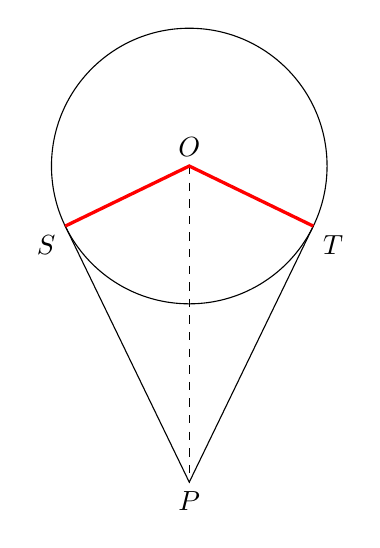
\begin{tikzpicture}[scale=0.35]
				\coordinate [label=above:$O$](O) at (0,0);
				\coordinate [label=below:$P$](P) at (0,-11.4707866935);
				\coordinate [label=below left:$S$](S) at (-4.5,-2.17944947177);
				\coordinate [label=below right:$T$](T) at (4.5,-2.17944947177);

				\draw (O) circle (5);
				\draw (P) -- (S) -- (O) -- (T) -- cycle;

				\uncover<2->{\tkzMarkRightAngle[size=0.75](P,S,O);}
				\uncover<2->{\tkzMarkRightAngle[size=0.75](P,T,O);}

				\uncover<4->{\draw [dashed] (O) -- (P);}

				\uncover<3->{\draw [red,very thick] (S) -- (O) -- (T);}
			\end{tikzpicture}
		\end{column}
		\begin{column}{0.6\textwidth}
			\begin{example}
				If $P$ is a point outside of a circle and $PT$ and $PS$ are two tangents to the circle, then the following are true:
				\pause
				\begin{enumerate}[<+->]
					\item A tangent at a point on a circle is perpendicular to the radius draw to the point.
					\item $PS = PT$: tangents to a circle from an external point are equal.
					\item $OP$ bisects the angle between the tangents.
				\end{enumerate}
			\end{example}
		\end{column}
	\end{columns}
\end{namedframe}
